\paragraph{Цель работы:}
Изучить краткие теоретические сведения по возможностям, приемам работы с программой Wireshark (файл netWS.pdf),
изучить типы фильтрации трафика, правила построения фильтров, приемы статистической обработки сетевого трафика в Wireshark.

Запустив Wireshark на захват, выполнить загрузку доступной в лабораторных условиях страницы (bstu.by, iit.bstu.by или др.).
Остановить и сохранить захват.
Для захваченных пакетов определить статистические данные:
\begin{enumerate}
    \item процентное соотношение трафика разных протоколов в сети
    \item среднюю скорость кадров/сек
    \item среднюю скорость байт/сек
    \item минимальный, максимальный и средний размеры пакета
    \item степень использования полосы пропускания канала (загрузку сети)
\end{enumerate}

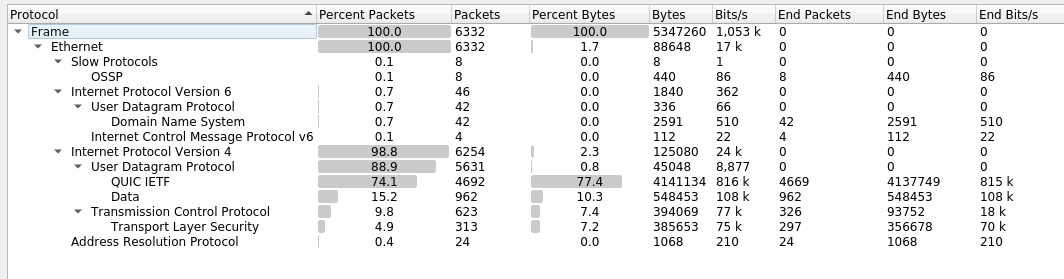
\includegraphics[width=0.9\textwidth]{resources/allProtocols}

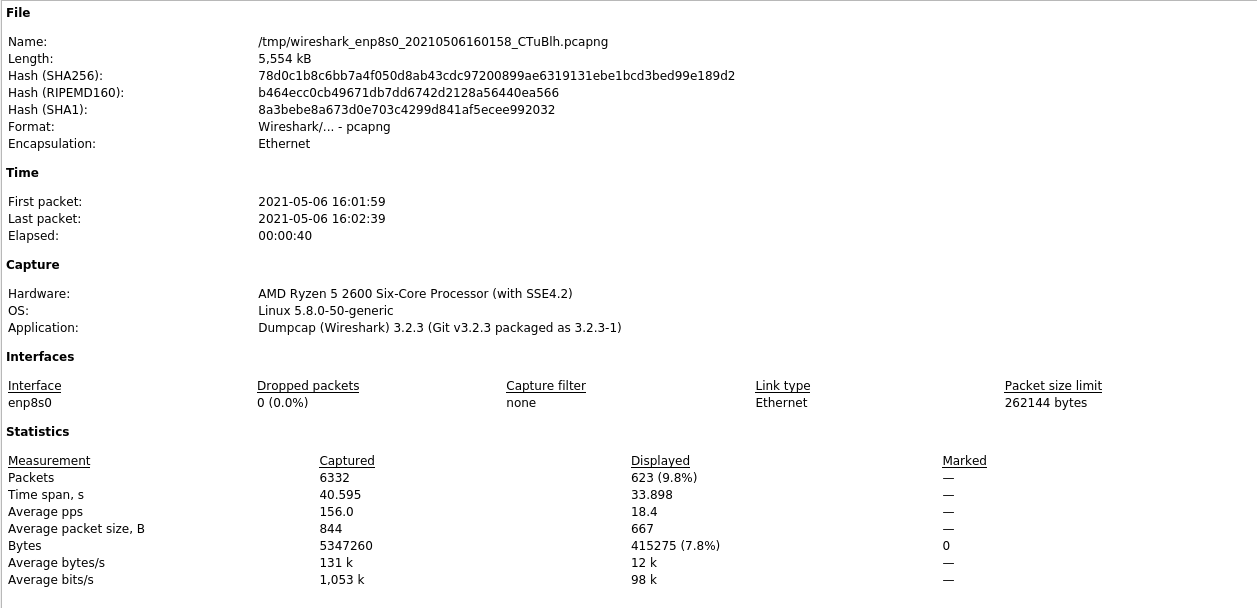
\includegraphics[width=0.9\textwidth]{resources/statisticBase}

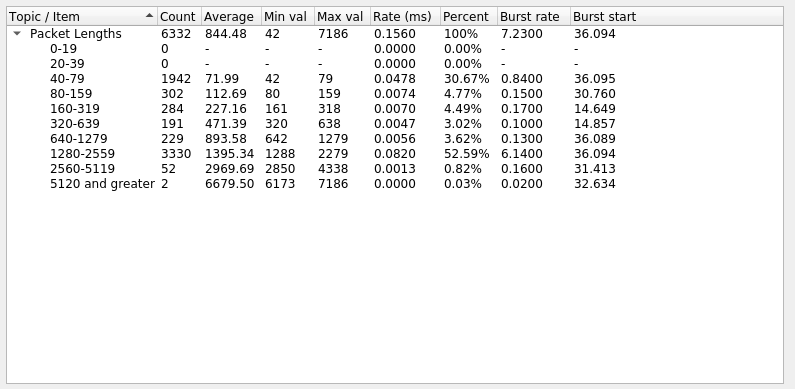
\includegraphics[width=0.9\textwidth]{resources/minMaxSize}

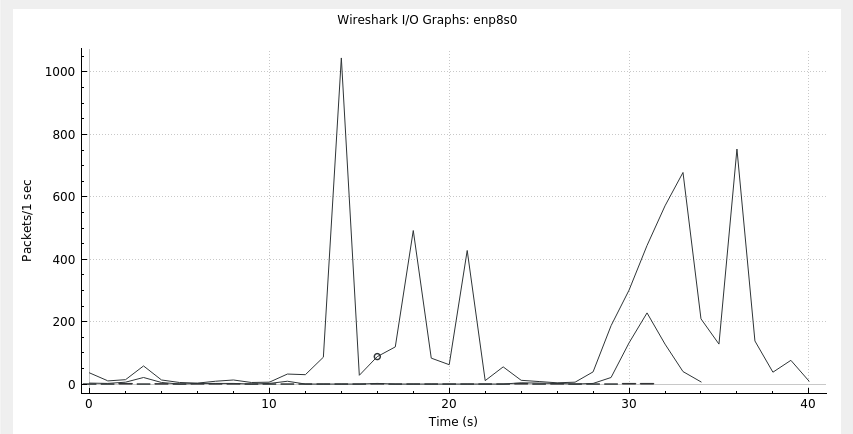
\includegraphics[width=0.9\textwidth]{resources/averageSpeed}

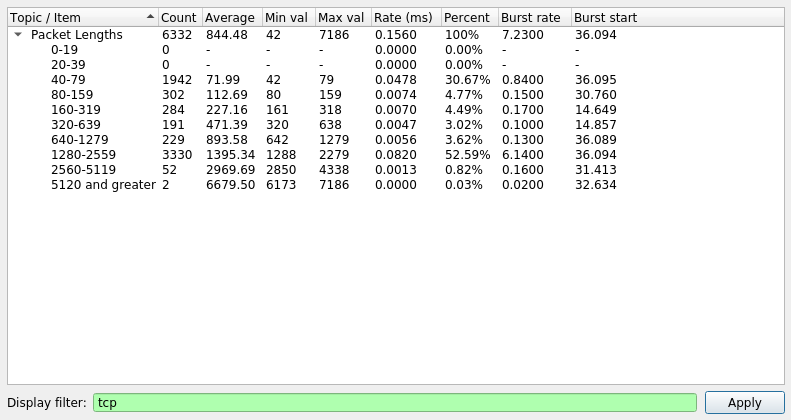
\includegraphics[width=0.9\textwidth]{resources/tcpAverageSize}

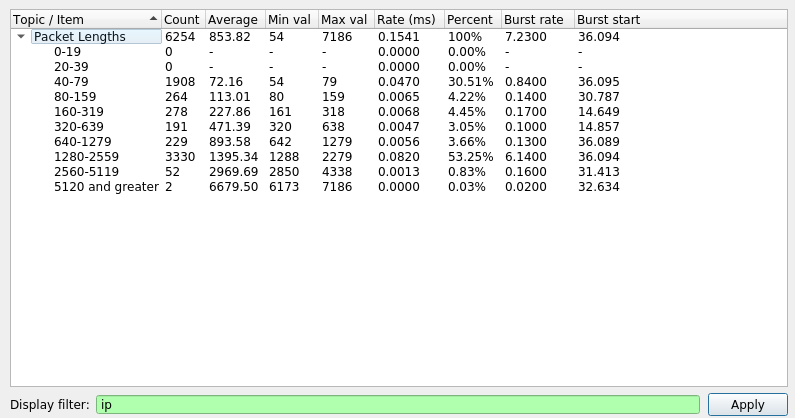
\includegraphics[width=0.9\textwidth]{resources/ipAverageSize}

На примере любого IP-пакета указать структуры протоколов Ethernet и IP.
Отметить поля заголовков и описать их и интерпретировать их значения.

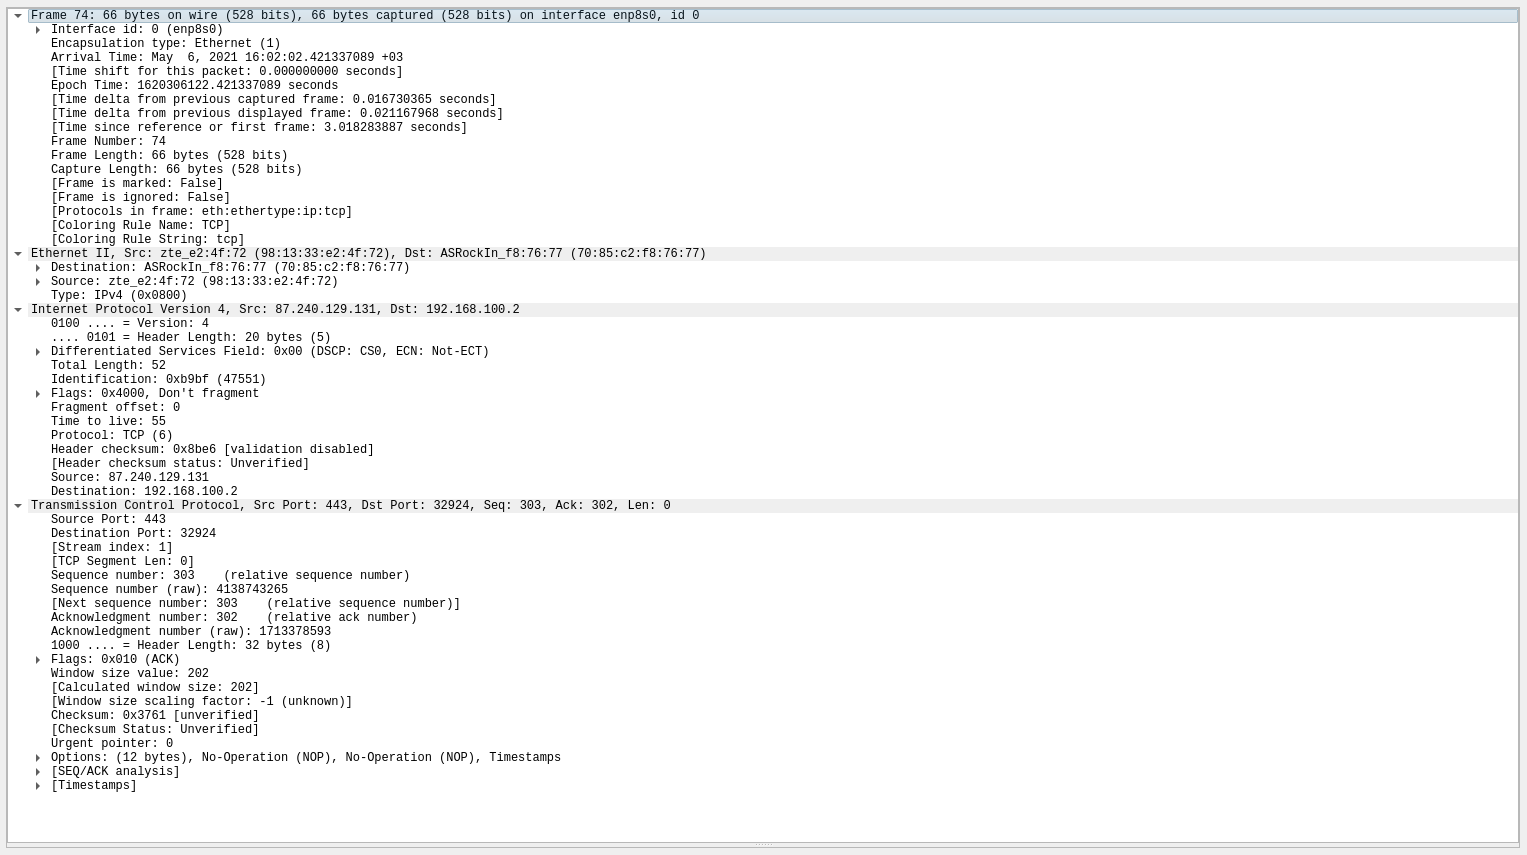
\includegraphics[width=0.9\textwidth]{resources/ipPackage}

\begin{itemize}
    \scriptsize
    \item Source --- физический адрес устройства отправителя.
    \item Destination --- физический адрес устройства получателя.
    \item Type --- тип протокола.
    \begin{itemize}
        \item Internet Protocol Version 4 - пакет протокола IPv4.
        \item Time to live: 64 – Максимально возможное количество сетевых устройств, которые могут обработать и передать пакет дальше по сети, равняется 64.
        \item Protocol: TCP (6) – На транспортном уровне используется протокол TCP.
        Значение данного поля позволяет устройству определить, какому протоколу транспортного уровня следует передать полученное PDU.
        В данном случае это протокол TCP.
    \end{itemize}
\end{itemize}

Запустив Wireshark на захват, выполнить команду ping для IP адреса соседней рабочей станции в лаборатории (предварительно определив ее адрес с помощью ipconfig).
Сохранить результат.
Сформировав нужный фильтр, отфильтровать пакеты, относящиеся к выполнению команды ping.
На базе полученных пакетов и значений их полей интерпретировать результат работы утилиты ping.
Описать все протоколы, используемые утилитой.
Составить диаграмму взаимодействия машин при работе утилиты ping.
Примечание.
Данная утилита использует протокол ICMP (RFC 792 и RFC 960).

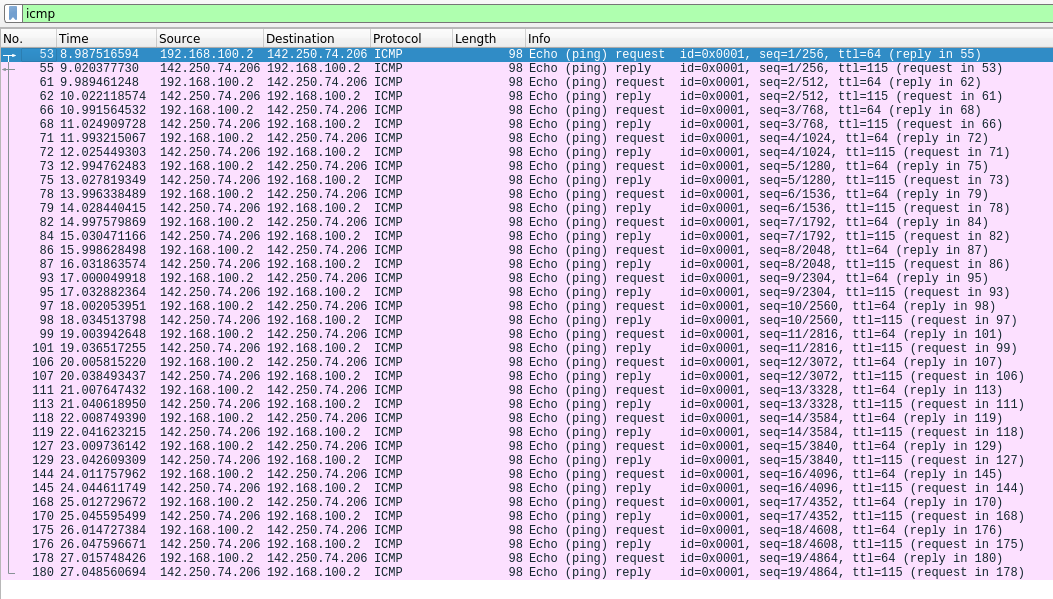
\includegraphics[width=0.9\textwidth]{resources/filterIcmp}

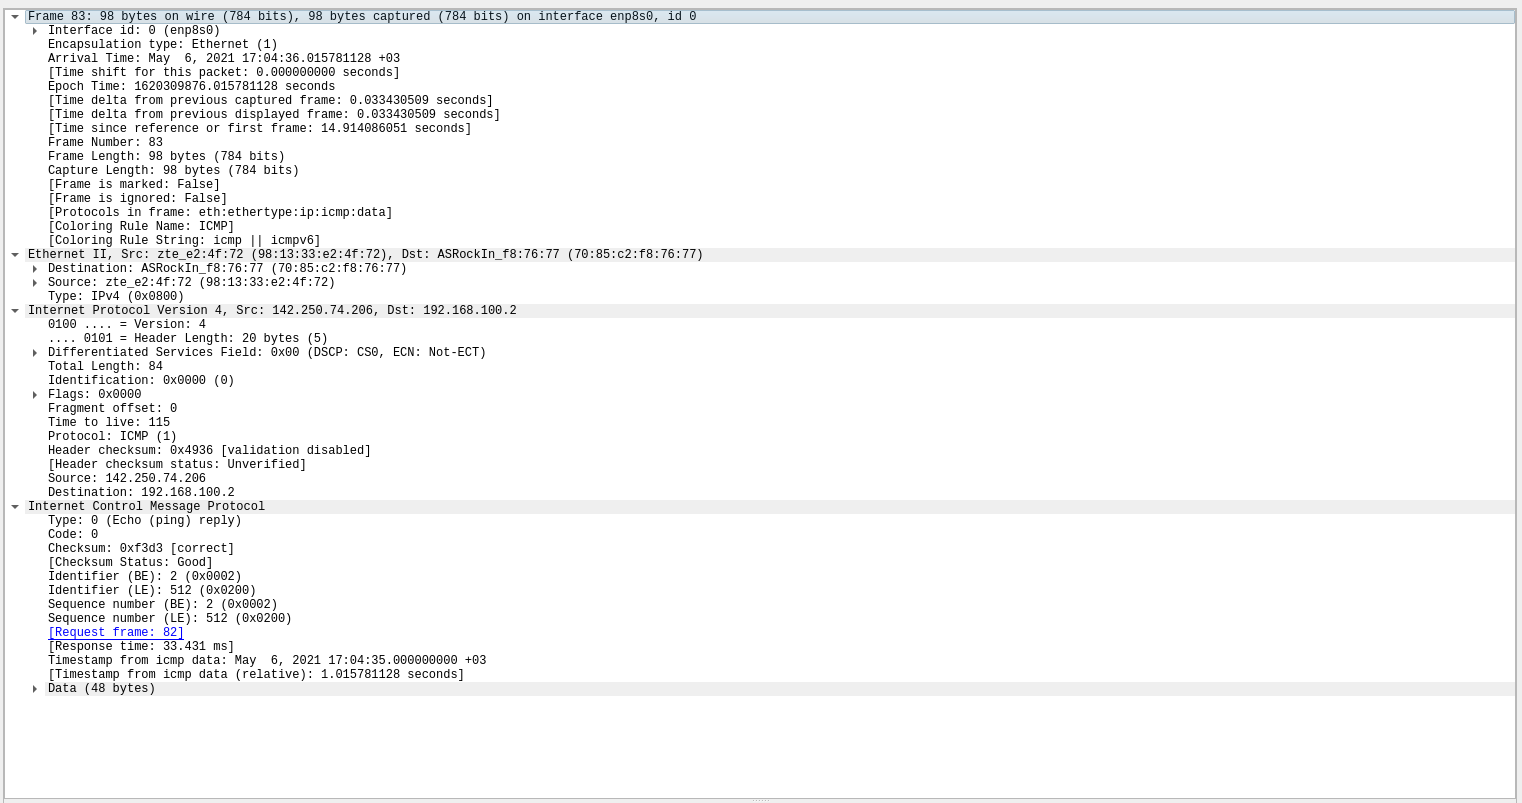
\includegraphics[width=0.9\textwidth]{resources/ping}

\begin{itemize}
    \scriptsize
    \item Type: 0 (Echo (ping) reply) - тип сообщения ICMP.
    \item 0 - эхо-ответ (Echo Replay).
    \item Checksum: 0xf3d3 [correct] - контрольная сумма, вычисляется из части ICMP пакета.
    \item Data (48 bytes) – поле данных
\end{itemize}

Выполнить анализ ARP-протокола по примеру из методических указаний.
ARP — сетевой протокол, предназначенный для преобразования IP-адресов (адресов сетевого уровня) в MAC-адреса (адреса канального уровня) в сетях TCP/IP.

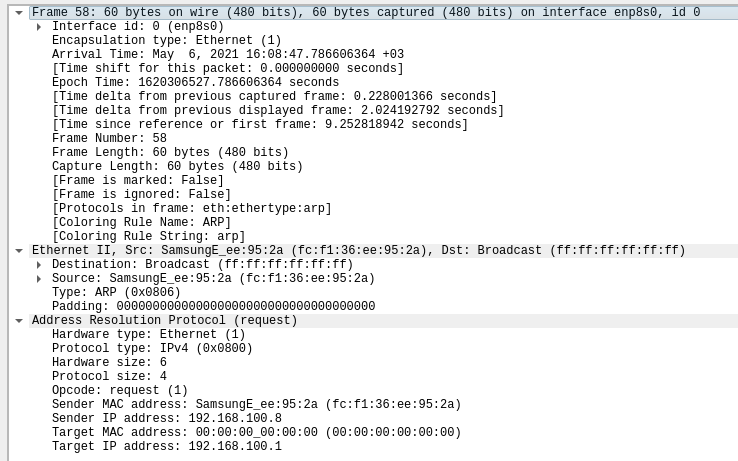
\includegraphics[width=0.9\textwidth]{resources/ARP}

\begin{itemize}
    \scriptsize
    \item Sender MAC address --- MAC-адрес отправителя.
    \item Sender IP address --- IP-адрес отправителя.
    \item Target IP address --- IP-адрес получателя.
\end{itemize}

